\chapter{人工智能对云计算的增强技术研究}
云计算中存在如下两个基本问题。第一,站在用户的视角,如何在浩如烟海的公有云资源池中选择最适合其应用程序的资源,即云配置优化问题。公有云厂商所提供的计算资源类型和计费模式越来越复杂。据不完全统计,截至目前,AWS EC2提供了超过400种配置的虚拟机,阿里云提供了超过500种虚拟机。除了虚拟机配置不同之外,其收费模型也存在多种。例如,除了传统的包年包月、按量付费等,还有抢占式实例(在AWS中成为Spot Instance)等计费方式。在此场景中,用户所面临的一个重要问题在于如何为自己的应用程序/负载选择合适配置和收费方式的资源。第二站在公有云运营商的角度,如何调度资源使其满足所有用户的需求,且达到一定的调度目标例如集群资源利用率最高、吞吐率最高等等。

近年来越来越多的学者尝试利用机器学习算法来解决上述两类问题。不同于前两章所述的公有云服务对机器学习负载的支持(Cloud for AI),本章将从“机器学习对云计算的增强技术”(AI for Cloud)着手,研究相关技术。
\section{基于机器学习算法的云资源配置优化技术}
自2010年AWS(Amazon Web Service)将云计算在产业界落地以来,各种云计算模型和应用层出不穷。云计算的高度弹性和海量的资源大大解放了开发者,使他们可以不用费时费力去关注数据中心的运维、物理节点的伸缩。受益于云计算的便捷性,公司、科研机构、事业单位都在将自己的负载向公有云上迁移。尽管云厂商提供了诸如IaaS、PaaS、SaaS、FaaS等各种云服务,但受限于绝大多数传统应用的架构和重构代价,大部分应用上云需求对准的都是基础的IaaS服务,即将部署在本地私有数据中心的应用迁移在云厂商提供的虚拟机上,以降低运维成本,并使原有的应用具备一定的弹性。

\begin{figure}[h]
    \centerline{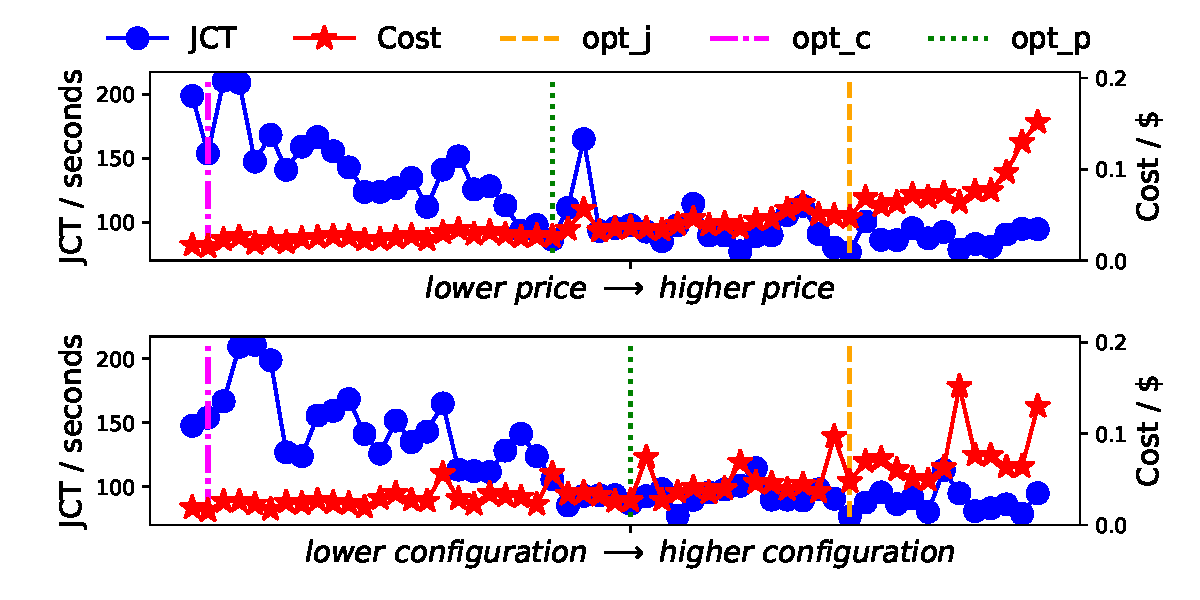
\includegraphics[width=\textwidth]{figures/mis_conf_effect.pdf}}
    \caption{同一任务在不同云配置下的性能和花费。}
    \label{mis_conf_effect}
\end{figure}

然而,即便云厂商帮助用户完成了集群维护、可靠性保障,但用户仍然需要在庞大的配置空间中选择最适合自己的应用和自己的需求的配置。而且,用户的需求各异,有的需要选择使得其应用完成时间尽可能短的配置,有的需要选择最终总花费尽可能少的配置,还有的可能综合考虑这两点,选择性价比最高的配置。如果仅凭一些启发式的规则,例如,选择配置最高的或者单价最低的,往往难以选择到最优的配置。图~\ref{mis_conf_effect}展示了Spark-Terasort这一任务在55种云资源配置上(跨越AWS、阿里云、腾讯云、华为云四大云厂商)的任务完成时间和总花费曲线。该图中,横轴代表不同的配置,其中上面的子图中,配置的单价由左到右单调递增,下面的子图中,配置的规则由左到右单调递增。opt\_j, opt\_c, opt\_p分别代表最优完成时间、最优花费和最优性价比,JCT为Job Completion Time的缩写,代表任务完成时间。很显然,最优的配置与直觉相违背。因此,此类用户需要一个自动选择最优配置的算法/工具,来帮助他们为自己的应用程序/负载选择最符合他需求(完成时间最短,总体花费最低或者性价比最高)的配置。

尝试解决此类问题的相关工作,其大体可以分为两类:1)数据驱动的线下建模方法;2)基于搜索的线上优化方法。本节按照这种分类方法介绍相关工作。

\subsection{数据驱动的线下建模方法}\label{sec_profling}

该类方法旨在通过在线下收集一系列形如 <meta data, performance> 的键值对,然后利用机器学习算法对上述键值对建立回归模型,以预测性能。其中meta data中可能既包括配置信息,如当前运行环境的硬件配置(CPU核数,CPU代数,memory大小等等),又包括可以刻画该workload的一些信息,如workload运行时某一时刻的CPU利用率等等。对于用户而言,使用该类算法的总体流程如图\ref{offline_profiling}所示。

\begin{figure}[h]
    \centerline{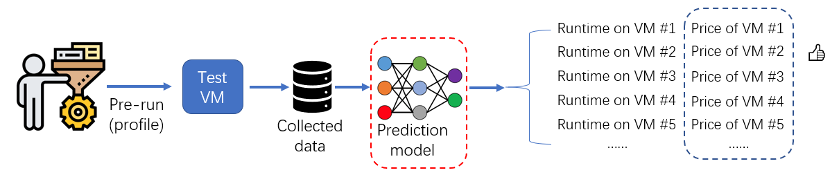
\includegraphics[width=\textwidth]{figures/offline_profiling.png}}
    \caption{数据驱动的线下建模方法流程图。}
    \label{offline_profiling}
\end{figure}

在模型训练阶段,需要对不同的workload在不同的VM上进行profile,形成形如<configuration, performance> 的键值对。然后对由该键值对构成的数据集进行模型训练。在预测阶段,用户需要在一个或者多个test VM上预运行自己的workload,并采集一些模型需要的数据,将其输入模型,并得到预测结果。该结果可能是该workload在配置集上所有VM配置上运行的性能数值或者最有的配置。总的来讲,该种类别中,不同的工作的主要区别在于上图中Prediction Model的结构。

\begin{figure}[h]
    \centerline{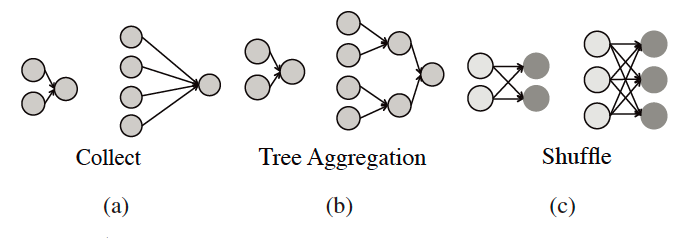
\includegraphics[width=\textwidth]{figures/ernest-data-flow.png}}
    \caption{Ernest中的三种数据流模式。}
    \label{ernest_data_flow}
\end{figure}

S. Venkataraman等人在2016年提出了Ernest\parencite{venkataraman2016ernest},可以称为云上性能建模的开山之作。Ernest主要关注Hadoop,Spark等基于map-reduce计算范式的应用程序。Ernest将基于map-reduce计算范式的程序中的数据流模式总结为如图~\ref{ernest_data_flow}所示的Collect、Tree Aggregation和Shuffle三种模式。其认为三种数据流模式的计算复杂度分别为$O(\frac{1}{machines})$,$O(machines)$和$O(log(machines))$, 因此使用公式~\ref{eq_ernest_model}对应用程序的性能进行拟合。虽然此模型非常简单,但是Ernest通过基于Spark-MLlib的实验证明了其模型可以达到较低的预测错误,且profile的代价较小。

\begin{equation}\label{eq_ernest_model}
    \begin{aligned}
    time =& \theta_0 + \theta_1 \times (scale \times \frac{1}{machines}) + \\
        &\theta_2 \times log(machines) + \\
        &\theta_3 \times machines
    \end{aligned}
\end{equation}

Ernest虽然可以达到较好的效果,但是其仅针对Hadoop和Spark等MR范式的应用,无法在一般性的场景中得到应用。且Ernest并未将资源配置作为输入参数,对于每种资源都需要使用模型建立一个单独的模型进行预测,在复杂的公有云中适用性较低。N. Yadwadkar等人在2017年提出了PARIS\parencite{yadwadkar2017selecting}。如图基于随机森林模型和两次预先运行收集到的数据对常用的数据处理任务进行性能建模。不同于Ernest,PARIS的输入参数除了资源信息,还包括预运行中收集到的关于当前应用程序的系统指标(最后一分钟、五分钟和十五分钟的系统指标,例如CPU利用率,内存利用率,中断次数等)。同时PARIS还不仅支持性能建模,还支持对花费进行建模。用户可以根据自己的需求,使用PARIS选择性能最优或者花费最低的云资源。

\begin{figure}[h]
    \centerline{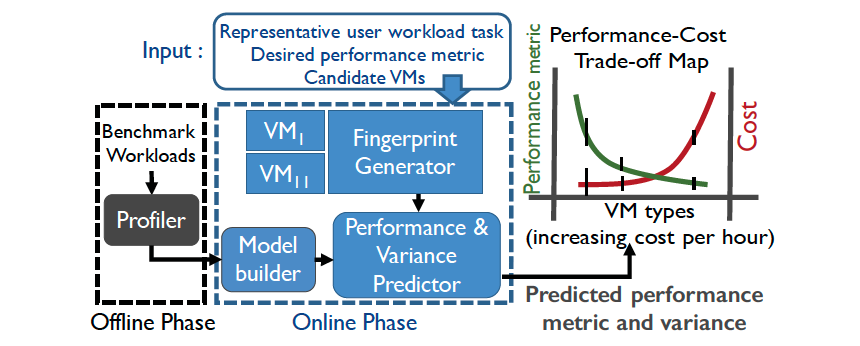
\includegraphics[width=\textwidth]{figures/paris-arch.png}}
    \caption{PARIS系统架构。}
    \label{paris_arch}
\end{figure}

从另一个角度来看,云资源的配置优化问题实际上可以视作推荐问题的一个变种,即在配置集合中为用户推荐最适合其应用程序的配置。A. Klimovic在2018年提出了Selecta\parencite{klimovic2018selecta},使用隐因子协同过滤算法为用户推荐合适的云资源配置。如图~\ref{selecta_arch}所示,Selecta先使用训练应用集在20\%的配置上预先运行,用户的目标应用需要在两个配置上预先做运行。上述运行得到的数据(任务完成时间或者最终花费)会形成一个行为不同配置列为不同应用程序的稀疏矩阵。然后Selecta利用SVD(特征值分解)对矩阵进行补全,最后根据最后一行推理出来的结果推荐出最优的配置。在该应用实际运行结束后,其运行结果会补充到该矩阵中以对数据进行增强,使模型的推荐效果更优。

\begin{figure}[h]
    \centerline{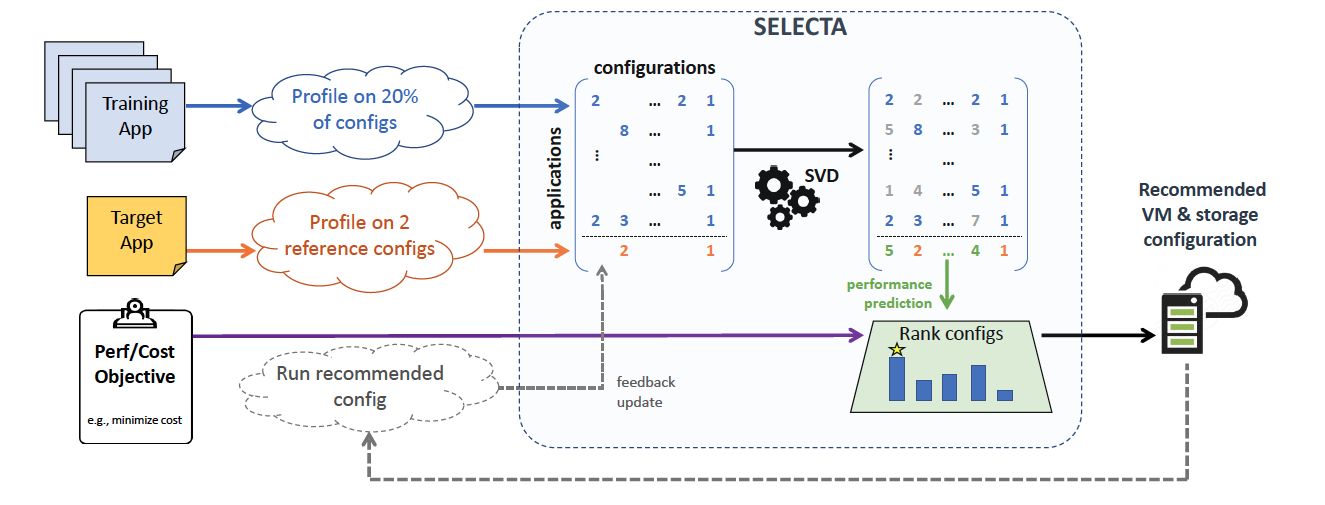
\includegraphics[width=\textwidth]{figures/selecta-arch.png}}
    \caption{Selecta系统架构。}
    \label{selecta_arch}
\end{figure}

随着深度学习模型的流行,也有研究者提出使用深度学习模型对应用性能进行建模,从而为应用选择最合适的云资源。F. Moradi\parencite{moradi2019performance}在2019年提出使用迁移学习算法实现通用的云应用性能预测。该方法先使用一个应用程序在所有的云配置上运行并收集性能数据,然后用深度神经网络对其建立性能模型,并将该模型计作基础模型。当需要为新的应用程序预测性能时,则抽出基础模型中的前若干层中的已训练参数放在新模型中,并使用新应用程序在少量配置上预运行得到结果对该模型进行微调,从而得到一个模型。该方法实际上是将已训练好的模型视作应用程序的特征抽取器,再使用其抽取的特征在新的数据上重新训练得到新模型。

基于上述工作,后续也有若干工作尝试在不同的应用场景下解决配置优化问题,但是总体上的方法皆大同小异。

\subsection{基于搜索的线上优化方法}
该类方法不同于数据驱动的线下建模方法,不需要在线下建立性能模型。其一般使用相关搜索算法(例如贝叶斯优化)在线上不断地搜索,并同时更新一个置信函数,当该函数值大于(或小于)某个阈值时,便停止搜索,用当前的到的数据中最优的一个作为结果。作为无需线下建模的纯线上方法,其固然具有其方便性。但是由于其掌握的信息过少,准确性一般要比基于线下建模的方式略低。

\begin{figure}[h]
    \centerline{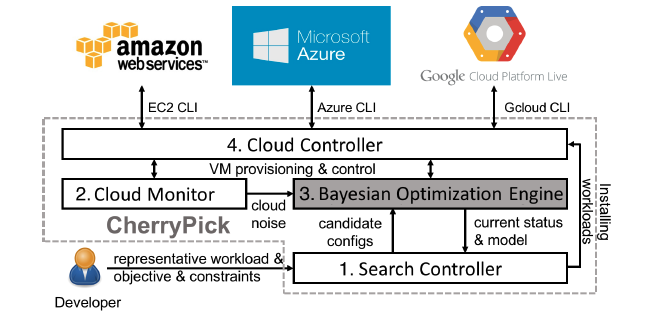
\includegraphics[width=\textwidth]{figures/cherrypick-arch.png}}
    \caption{CherryPick系统架构。}
    \label{cherrypick_arch}
\end{figure}

O. Alipourfard等人在2016年提出CherryPick\parencite{alipourfard2017cherrypick},使用典型的BO(Bayes Optimization,即贝叶斯优化)持续搜索不同的配置,直到其定义的置信函数超过某个阈值,则将当前搜索到的最优值作为最后的结果。图~\ref{cherrypick_arch}描述了CherryPick的系统架构,其支持在AWS,Azure和Google Cloud三家云厂商中对资源进行搜索,且支持用户自定义搜索的目标函数。

在CherryPick基础上,M. Casimiro等人在2020年提出了Lynceus\parencite{casimiro2019lynceus}。有别于CherryPick,Lynceus没有使用贪心的搜索方法,且不需要事先了解目标应用程序的任何信息。图~\ref{lynceus_arch}阐述了Lynceus与传统贝叶斯优化方法的区别所在。首先,Lynceus在考虑每一次搜索的reward的同时,还考虑了这一次搜索可能造成的cost。其实,传统的贝叶斯优化在一次尝试后即根据反馈推断下一次搜索的配置,Lynceus则是先预估一个可能的搜索路径,然后对路径的第一个节点进行尝试,最后得到最优结果。Lynceus更远的视野和更为精细的回报函数设计使得其相比于传统的贝叶斯优化拥有更高的准确率。

\begin{figure}[h]
    \centerline{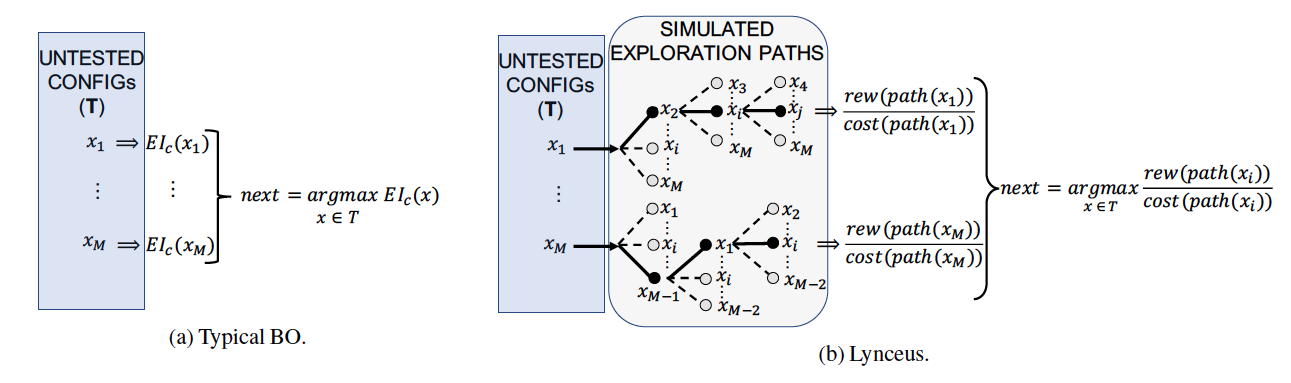
\includegraphics[width=\textwidth]{figures/lynceus-arch.png}}
    \caption{Lynceus与传统贝叶斯优化的区别。}
    \label{lynceus_arch}
\end{figure}

\section{基于机器学习算法的云资源调度优化技术}
资源调度是操作系统、分布式系统和云计算领域中的经典问题,其本质在于为系统中的每个任务分配合适的资源,从而使得系统达到某种状态,如资源利用率最高、闲置资源最少或者吞吐率最高等。近年来越来越多的学者开始尝试使用机器学习算法,特别是深度学习算法,对调度问题进行建模,试图更精确地解决调度问题。

C. Delimitrou等人在2014年提出了Quasar\parencite{delimitrou2014quasar},旨在保证作业性能的同时提升云上集群的资源利用率。Quasar和目前云计算厂商使用的资源预留策略(用户申请一定量的资源后即按照该量分配,即时相当一部分分配的资源处于空载状态)不同,而是要求用户提供一个动态的目标,使得集群调度器可以动态地适配其需要的资源。图~\ref{quasar_arch}展示了Quasar的系统架构。Quasar使用了协同过滤算法得到workload在满足QoS的前提下需要的资源数量和类型,以及会与那些workload产生干扰,再利用这一结果贪心地分配资源。通过实验,Quasar在200个EC2服务器的集群环境中提高了47\%的资源利用率。

\begin{figure}[h]
    \centerline{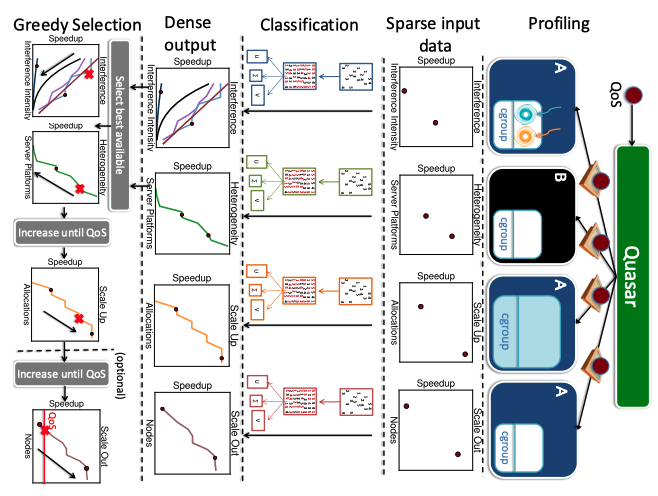
\includegraphics[width=\textwidth]{figures/quasar架构.png}}
    \caption{Quasar架构示意图。}
    \label{quasar_arch}
\end{figure}

随着深度学习的进一步发展,也有许多工作尝试将强化学习应用于调度问题。强化学习( Reinforcement Learning )是一种机器学习方法。这种方法通过与环境不断交互获得交互的反馈,从而获得经验,再从经验中不断学习,最终获得最优策略。其中经验(experience)是与环境交互得到的状态state)、动作action)和收益reward的采样序列。

H. Mao等人在2019年提出了Decima\parencite{mao2019learning},利用message passing等方法,将DAG作业的图结构建模到神经网络中,从而使得神经网络模型具有可扩展性,可适应任意作业队列长度的输入,而后通过policy gradient等强化学习方法训练调度器。结果显示Decima相比之前的启发式调度算法至少减少了21\%的平均作业完成时间。

除了使用强化学习算法,Decima中的另一个核心思想是使用图神经网络将DAG图中的作业节点编码成向量(亦称作embedding),再由这些向量生成Job级别的embedding和全局的embedding。这种思想借鉴于自然语言处理中的word2vec和图神经网络中的node2vec。如图~\ref{decima_embedding}所示,embedding生成的依据是DAG中各个节点之间的依赖关系。这样做的好处是将图中节点的依赖关系转化为高维空间中向量之间的代数关系,使得模型能够更容易的学习到规律。

\begin{figure}[h]
    \centerline{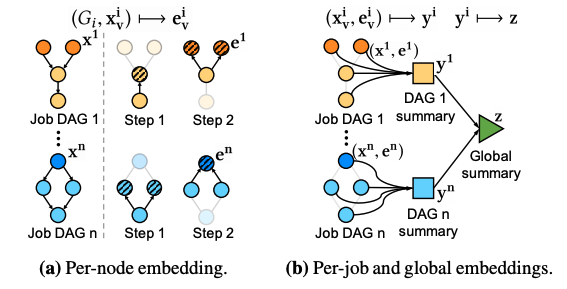
\includegraphics[width=\textwidth]{figures/decima-embedding.png}}
    \caption{Decima中的embedding生成示意图。}
    \label{decima_embedding}
\end{figure}

F. Li等人在2019年提出了DeepJS\parencite{li2019deepjs},将问题模型化为选择机器-作业对的问题,每次调度前构造可行的机器作业对列表,由神经网络输出每个对的得分,优先调度得分高的机器作业对。A. Mirhoseini等\parencite{mirhoseini2017device}使用强化学习算法训练了Tensorflow计算操作的放置策略(放置于哪个计算设备,如CPU),它使用了一种循环神经网络去编码状态,而不是采用具有可扩展性的图神经网络。

\begin{figure}[h]
    \centerline{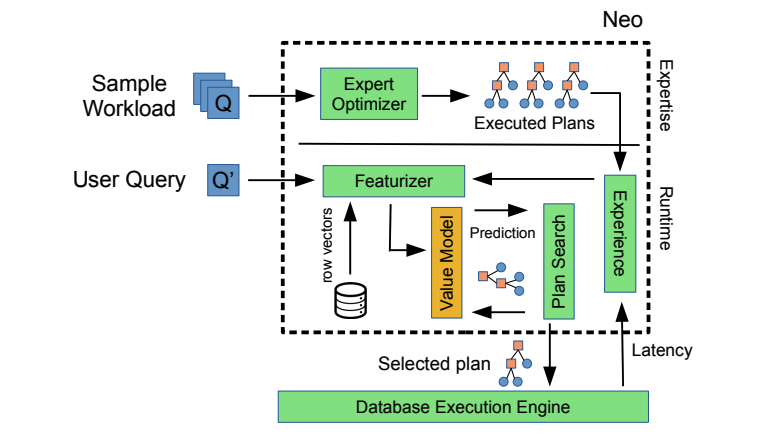
\includegraphics[width=\textwidth]{figures/neo-arch.png}}
    \caption{Neo系统架构示意图。}
    \label{neo_arch}
\end{figure}

受到Decima的启发,有一些学者开始考虑将深度学习算法和图神经网络应用到云数据库中的查询优化中,因为数据库中的一次查询所对应的语法树天生就是一个DAG图,图的节点对应数据库中的operator。R. Marcus等人在2019年提出Neo\parencite{marcus2019neo},一种基于深度学习的数据库查询优化器。图~\ref{neo_arch}阐述了Neo的系统架构。与~\ref{sec_profling}中所述的基于线下模型训练的性能预测方法类似,Neo需要先使用sample workload,通过一个已有的最优优化器(可能是基于专家的经验,也可能基于历史信息),构建一个查询优化的信息库(即图中的Experience)。当用户发起查询时,Neo中的特征提取器会结合经验和用户的查询语句对其进行特征提取。此处的特征提取Neo使用了树形的卷积网络对语句中的operator进行编码,然后做出决策,交由数据库引擎执行。T. Kraska在2019年也提出了一个基于深度学习的数据库系统SageDB\parencite{47669}。和Neo相比,SageDB更进一步,其在数据库查询执行、数据预取等阶段都利用机器学习模型做了相关优化

\section{小结}

本节从用户和云厂商运营者两个角度,研究了云计算中的两个经典问题,即云资源配置优化与云资源调度。基于机器学习的云资源配置优化技术正在经历从支持特定领域应用向支持通用应用的发展历程。未来,关于如何用较小的代价获取通用性较强的资源配置优化模型,将会是研究的重点。基于机器学习的资源调度算法一般都是将资源调度问题抽象为典型的机器学习领域的问题,例如通过协同过滤算法建立不同实体之间的关系,利用图神经网络对DAG图的节点进行编码,利用强化学习不断调整系统的状态等等。事实上,利用机器学习算法解决调度问题目前亦处于探索阶段。大型分布式系统中,往往要求调度器能够快速做出决策,而基于机器学习尤其是深度学习的调度模型,往往具有较高的延时,可能会给系统带来过重的额外开销。未来,除了使调度算法做出更优的决策之外,尝试降低基于ML的调度算法的额外开销,也会是一个可能的研究方向。